\chapter{Preliminaries}\label{chap:preliminaries}

\section{SAT basics}

\subsection{Satisfiability problem}
A \emph{Boolean variable}, or \emph{propositional variable}, is a variable that
has two possible values : true or false (noted respectively $\true$ or $\false$).
A \emph{literal} $l$ is a propositional variable or its
negation. For a given variable $x$, the positive literal is represented by $x$
and the negative one by $\neg x$.
A \emph{clause} $\omega$ is a finite disjunction of literals represented
equivalently by $\omega = \bigvee_{i=1}^k l_i$ or the set of its literals
$\omega = \{l_i\}_{i \in \llbracket 1,k \rrbracket}$. A clause with a single
literal is called \emph{unit clause}.
A clause is a \emph{tautology} if it is always true, a clause that contains a positive 
and negative value of a clause for example.
A \emph{conjunctive normal form (CNF) formula} $\varphi$ is a finite
conjunction of clauses.  A CNF can be either noted $\varphi = \bigwedge_{i=1}^k
\omega_i$ or $\varphi = \{\omega_i\}_{i \in \llbracket 1,k \rrbracket}$. We
denote $\Vars_\varphi$ ($\Lits_\varphi$) the set of variables (literals) used in
$\varphi$ (the index in $\Vars_\varphi$ and $\Lits_\varphi$ is usually omitted when
clear from context).

For a given formula $\varphi$, an \emph{assignment} of the variables of
$\varphi$ is a function $\alpha: \Vars \mapsto \{ \true, \false \}$.  As usual, $\alpha$ is
\emph{total}, or \emph{complete}, when all elements of $\Vars$ have an image by
$\alpha$, otherwise it is \emph{partial}. By abuse of notation, an assignment is
often represented by the set of its true literals.  The set of all (possibly
partial) assignments of $\Vars$ is noted $\Assignments(\Vars)$.

The assignment $\alpha$ \emph{satisfies} the clause $\omega$, denoted $\alpha
\models \omega$, if $\alpha \cap \omega \neq \emptyset$. Similarly, the assignment
$\alpha$ satisfies the propositional formula $\varphi$, denoted $\alpha \models
\varphi$, if $\alpha$ satisfies all the clauses of $\varphi$. Note that a
formula may be satisfied by a partial assignment. In this case, unassigned variable are called
\emph{dont care}.
A formula is said to be
\emph{satisfiable} (\sat) if there is at least one assignment that satisfies it;
otherwise the formula is \emph{unsatisfiable} (\unsat).

\subsection{An NP-complete problem}

The SAT problems is the first NP-complete algorithm as proven by Stephen Cook in 1971~\cite{cook1971complexity}.
NP-completeness means that a SAT problem can be solved with a non deterministic machine in polynomial time (NP) and is also NP-hard. A problem is said NP-hard if everything in NP can be transformed into it in polynomial time. 
One of the most important unsolved problem in theoretical computer science is the P versus NP problem.
This question is one of the seven millennium prize problems.

Some particular form of the SAT problems can be computed in linear time for 2-SAT~\cite{aspvall1979linear}
where each clause is in binary form i.e. size  of two. %This kind of clauses can be written as implication 
Others particular form  can be solved in  polynomial time like Horn SAT~\cite{aspvall1979linear} in which it suffice to  apply \emph{unit propagation} explained in \cref{sec:dpll} until fix point.
Xor-SATisfiability where each clause contains exclusive or belong also to the polynomial class.

%It asks if every problems can be solved and verified in polynomial time.
%Any NP problems can be reduced in polynomial time by a deterministic Turing machine to the SAT problems.
%The states that the propositional satisfiability problem is NP-complete
%SAT is NP because any assignment of Boolean values to Boolean variables that is claimed to 
%satisfy the given expression can be verified in polynomial time by a deterministic Turing machine. 
%
%


\subsection{Solving a SAT problem}

Two kinds of algorithm exists to solve satisfiability problems.
First, the \emph{incomplete} algorithm which does not provide any guarantee that will eventually report either any satisfiable assignment or declare that formula is unsatisfiable. This kind of algorithm is out of scope of this thesis. 
Second, the \emph{complete} algorithm, which provides a guarantee that if an assignment exists
it will be reached or it will declare that formula is unsatisfiable.
This section describes different \emph{complete }algorithm to solve a propositional formula.



\subsubsection{A naive algorithm}
A naive approach to solve a SAT problem is to try all possible assignments. In total,
for a propositional formula with $n$ variables, it leads to $2^n$ assignments in the worth case.  
\Cref{fig:naive_algo} illustrate the search tree for a given problem with six variables.
In this case $\alpha_{11}$ ($\neg x_1, \neg x_2, x_3, \neg x_4, x_5, \neg x_6 $) is found as a solution of the problem. In the general case,
this algorithm is obviously intractable on real problems even for a formula with few variables.


\begin{figure}[!htbp]
	\centering
	
\begin{minipage}[c]{0.6\linewidth}
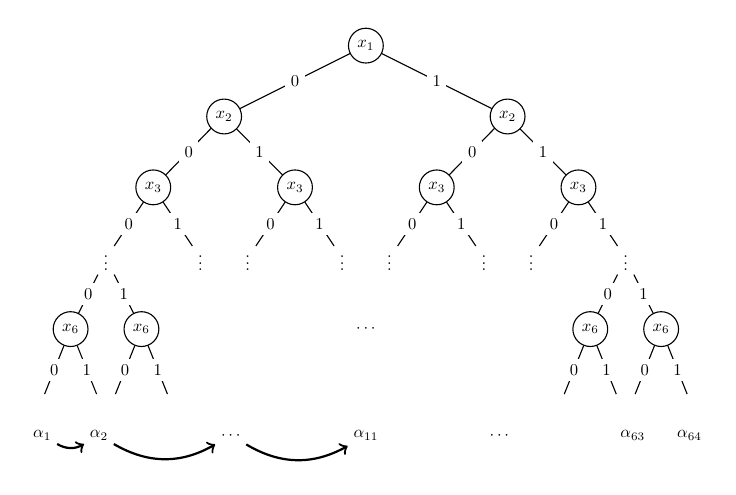
\begin{tikzpicture}[level/.style={sibling distance=60mm/#1},every node/.style={scale=0.6}, scale=0.6]
  \tikzstyle{trans}=[thick, ->, sloped]

\node [circle,draw] (x1) {$x_1$}
  child {node [circle,draw] (x2_1) {$x_2$}
    child {node [circle,draw] (x3_1) {$x_3$}
      child {node  (xn_1) {$\vdots$}
        child {node [circle,draw] (x6_1) {$x_6$}
        	child {node (x6_1f) {}
        	child[level distance=0.75cm] { node (a1) {$\alpha_1$} edge from parent[draw=none]}
        }
       		child {node (x6_1t) {}
       			child[level distance=0.75cm] { node (a2) {$\alpha_2$} edge from parent[draw=none]}
         }}
        child {node [circle,draw] (x6_2) {$x_6$}
        		child {node (x6_2f) {}}
        				child {node (x6_2t) {}
        	}
        }
      } 
      child {node (xn_2) {$\vdots$}}
    }
    child {node [circle,draw] (x3_2) {$x_3$}
      child {node (xn_3) {$\vdots$}}
      child {node (xn_4) {$\vdots$}}
    }
  }
  child {node [circle,draw] (x2_2) {$x_2$}
    child {node [circle,draw] (x3_3) {$x_3$}
      child {node (xn_5) {$\vdots$}}
      child {node (xn_6) {$\vdots$}}
    }
  child {node [circle,draw] (x3_4) {$x_3$}
    child {node (xn_7) {$\vdots$}}
    child {node (xn_8) {$\vdots$}
      child {node [circle,draw] (x6_3) {$x_6$}
      	       child {node (x6_3f) {}}
      	child {node (x6_3t) {}
        }}
      child {node [circle,draw] (x6_4) {$x_6$}
      	child {node (x6_4f) {}
        child[level distance=0.75cm] { node (an_1) {$\alpha_{63}$} edge from parent[draw=none]}
    	}
	    child {node (x6_4t) {}
    		child[level distance=0.75cm] { node (an) {$\alpha_{64}$} edge from parent[draw=none]}
      }}}
  }
};

\path (x6_2) -- (x6_3) node (x) [midway] {$\cdots$}
        child[level distance=2.25cm] { node (a_11) {$\alpha_{11}$} edge from parent[draw=none]};


\path (a2) -- (a_11) node (b1) [midway] {$\cdots$};
\path (a_11) -- (an_1) node (b2) [midway] {$\cdots$};

\draw[trans] (a1) to [bend right]  (a2);
\draw[trans] (a2) to [bend right]  (b1);
\draw[trans] (b1) to [bend right]  (a_11);

% to [bend right]  (b1) to [bend right]  (a_11);

\path (x1)   -- (x2_1) node [midway, fill=white] {$0$};
\path (x2_1) -- (x3_1) node [midway, fill=white] {$0$};
\path (x3_1) -- (xn_1) node [midway, fill=white] {$0$};
\path (xn_1) -- (x6_1) node [midway, fill=white] {$0$};
\path (x3_2) -- (xn_3) node [midway, fill=white] {$0$};
\path (x2_2) -- (x3_3) node [midway, fill=white] {$0$};
\path (x2_2) -- (x3_4) node [midway, fill=white] {$1$};
\path (x1)   -- (x2_2) node [midway, fill=white] {$1$};
\path (xn_1) -- (x6_2) node [midway, fill=white] {$1$};
\path (x3_1) -- (xn_2) node [midway, fill=white] {$1$};
\path (x2_1) -- (x3_2) node [midway, fill=white] {$1$};
\path (x3_2) -- (xn_4) node [midway, fill=white] {$1$};
\path (x3_3) -- (xn_5) node [midway, fill=white] {$0$};
\path (x3_3) -- (xn_6) node [midway, fill=white] {$1$};
\path (x3_4) -- (xn_7) node [midway, fill=white] {$0$};
\path (x3_4) -- (xn_8) node [midway, fill=white] {$1$};
\path (xn_8) -- (x6_3) node [midway, fill=white] {$0$};
\path (xn_8) -- (x6_4) node [midway, fill=white] {$1$};


\path (x6_1) -- (x6_1f) node [midway, fill=white] {$0$};
\path (x6_1) -- (x6_1t) node [midway, fill=white] {$1$};

\path (x6_2) -- (x6_2f) node [midway, fill=white] {$0$};
\path (x6_2) -- (x6_2t) node [midway, fill=white] {$1$};

\path (x6_3) -- (x6_3f) node [midway, fill=white] {$0$};
\path (x6_3) -- (x6_3t) node [midway, fill=white] {$1$};

\path (x6_4) -- (x6_4f) node [midway, fill=white] {$0$};
\path (x6_4) -- (x6_4t) node [midway, fill=white] {$1$};

\end{tikzpicture}
\end{minipage}
\begin{minipage}[c]{0.23\linewidth}
           \footnotesize
		\begin{itemize}
			\item[] $\omega_1 = \{x_1, x_2, x_3\}$ 
			\item[] $\omega_2 = \{x_4, x_5, x_6\}$
			\item[] $\omega_3 = \{\neg x_1, \neg x_5\}$
			\item[] $\omega_4 = \{\neg x_2, \neg x_4\}$
			\item[] $\omega_5 = \{\neg x_3, \neg x_4\}$
			\item[] $\omega_6 = \{\neg x_3, \neg x_6\}$
		\end{itemize}
\end{minipage}

	\caption{All possible assignments for a problem with 6 variables}
	\label{fig:naive_algo}
\end{figure}


\subsubsection{Davis Putnam Logemann Loveland (DPLL) algorithm}\label{sec:dpll}

One of the first non memory intensive algorithm to solve the SAT problems is 
the Davis Putnam Logemann Loveland (DPLL) algorithm~\cite{dpll_62}. 
It explores a binary tree using depth first search as given in \Cref{algo:dpll}.
The construction of the tree is related to a \emph{decision} literal (\cref{algo:dpll:decision}) then,
recursive call with each value are checked.
When a leaf report \unsat (\cref{algo:dpll:unsatbranch}), other branches are explored.
By recursive construction of the algorithm, when positive and negative value of a literal reach \unsat,
solver \emph{backtracks} at most one level, this fact is called \emph{chronological backtracking}.
If all leaves report $\unsat$  the formula $\varphi$ is unsatisfiable \cref{algo:dpll:unsat}.
Finally, if any branch found a solution  i.e. the problem is empty,
formula is satisfiable corresponding assignment is returned (\cref{algo:dpll:sat1,algo:dpll:sat2})

\begin{algorithm}[!htbp]
	\SetKwProg{Fn}{function}{}{}
	\SetKwFunction{DPLL}{DPLL}	
	\SetKwFunction{unitPropagation}{unitPropagation}
	\SetKwFunction{purePropagation}{purePropagation}
	\SetKwFunction{assignDecisionLiteral}{assignDecisionLiteral}

	
	\Fn{
		\DPLL{$\varphi$: CNF formula, $\alpha$ assignment}\\
		$\quad\quad$\textbf{returns} an assignment if $\varphi$ is \sat and $\unsat$ otherwise
	}
	{	
		$\varphi, \alpha \gets$ \unitPropagation{$\varphi, \alpha$}\;
	\label{algo:dpll:unit}
		\If{$\{\} \in \varphi$}{\Return \false \tcp*{Conflict}}	 \label{algo:dpll:unsatbranch}
		
		\If{$\varphi = \{\}$}{\Return $\alpha$ \tcp*{$\varphi$ is $\sat$}}
		
		$x \gets$ \assignDecisionLiteral{}\; \label{algo:dpll:decision}

		\If{$\alpha \gets$ \DPLL{$\varphi \cup \{x\}, \alpha $} \label{algo:dpll:pos}} 
		{
			\Return $\alpha$ 		\label{algo:dpll:sat1}
		}
		\If{ $\alpha \gets$ \DPLL{$\varphi \cup \{\neg x\}, \alpha $} \label{algo:dpll:neg}}
		{
			\Return $\alpha$ 		\label{algo:dpll:sat2}
		} 
	
		\Return \unsat \tcp*{$\varphi$ is $\unsat$}\label{algo:dpll:unsat}
	}
	\caption{The DPLL algorithm.}
	\label{algo:dpll}
	
\end{algorithm}

An important function in the DPLL algorithm is \texttt{unitPropagation} \cref{algo:dpll:unit} and
it is detailed in \Cref{algo:unitdpll}. It searches all unit clauses, then, to ensure satisfiability these literals must be true
and added to the current assignment. Formula is then simplified as follow, clauses that contains this literal are already satisfied
and can be deleted; negative literals are removed from the clause that belongs to him.
This procedure ends when either no unit clause remains or an inconsistency was found (empty clause).


\begin{algorithm}[!htbp]
	\SetKwProg{Fn}{function}{}{}
	\SetKwFunction{unitPropagation}{unitPropagation}
	\Fn{
		\unitPropagation{$\varphi$: CNF formula, $\alpha$ assignment}\\
		$\quad\quad$\textbf{returns}  CNF formula and assignment $\alpha$ 
	}
	{	
		\While{$\{l\} \in \varphi$ \textbf{and} $\{\} \notin \varphi$  }
		{
			\tcp{\small Remove all clauses containing $l$, all literals $\neg l$}
			$\varphi \gets \varphi\mid_{\,l}$\\
			$\alpha \gets \alpha \cup \{l\}$

		}
	\Return $\varphi, \alpha$
	}
	\caption{Unit propagation}
	\label{algo:unitdpll}
	
\end{algorithm}

When DPLL algorithm is executed on the formula in \Cref{fig:naive_algo}, after the decision of literal
$\neg x_1$ and $\neg x_2$ unit propagation detects that $x_3$ must be true. This propagation prevents to 
explore assignments from $\alpha_1 $ to $\alpha_{8}$. Moreover, application to unit propagation provokes more unit clauses
and leads directly to a solution. 
An important part of efficiency of DPLL is due to choose the variable that divide the search tree made by
the procedure \texttt{assignDecisionLiteral} . The objective of this function 
is to find a literal that will generate a maximum of unit propagation. Intuitively, decision literals 
can be viewed as "guesses" and propagated literals can be viewed as "deductions". Finding a optimal variable
is NP-Hard. Different heuristics exists to choose the decision variable,
some of them will be presented in section~\ref{sec:heuristics}.


%\input{algo/puredpll}
%Another idea introduced by DPLL was \emph{elimination of pure literals},
%a literal is said pure if it only appear on one sign (positive or negative) in the problem.
%These literals are set to true in the assignment.
%On consequence, all clauses that own these literals are satisfied and so can be removed.
%
\subsubsection{Conflict Driven Clause Learning (CDCL) algorithm}

The principal weakness of DPLL algorithm is to make same inconsistencies several times
(principally due to chronological backtracking), incurring unnecessary CPU usage.\\
Conflict Driven Clause Learning (CDCL) \cref{algo:cdcl} is another sound and complete algorithm
to resolve a SAT problem and overcome principal weakness of DPLL.


\Cref{algo:cdcl} gives an overview of CDCL, Like DPLL,  it walks on a binary search tree.
Initially, the current assignment is empty and decision level that indicated the depth of the search tree noted as $dl$ is set to zero.
Algorithm first applies unit propagation to the formula $\varphi$ for the current assignment $\alpha$ (\cref{alg:cdcl:unit}).
Note that it is exactly the same procedure as the one used for DPLL.
An inconsistency or a \emph{conflict} at level zero indicates that the formula is unsatisfiable, and the algorithm
reports it (\cref{alg:cdcl:unsat_start,alg:cdcl:unsat_end}). When the conflict is occurring at a higher level, it
reason was analyzed and a clause called \emph{conflict clause} is deduced (\cref{alg:cdcl:analyze}).
This clause is \emph{learnt} (\cref{alg:cdcl:learn}) (added to the formula). This clause is redundant from the current
formula and so as it does not change the satisfiability of $\varphi$. It also avoids encountering a conflict with the same
causes in the future. Working of this function will be presented thereafter.
The analysis is completed by the computation of a \emph{backjump}, solver unassign some literals and decrease
the decision level (\cref{alg:cdcl:backjump}). As the level can be much lower than the current assignment this is called 
\emph{non chronological backtracking}.
Finally, if no conflict appears, the algorithm chooses a new decision literal 
(\cref{alg:cdcl:pick_start,alg:cdcl:pick_end}).
The above steps are repeated until the satisfiability status of the
formula is determined.

\begin{algorithm}
	\SetKwProg{Fn}{function}{}{}
	\SetKwFunction{CDCL}{CDCL}
	\SetKwFunction{unitPropagation}{unitPropagation}
	\SetKwFunction{analyzeConflict}{analyzeConflict}
	\SetKwFunction{addLearntClause}{addLearntClause}
	\SetKwFunction{assignNewLiteral}{assignDecisionLiteral}
	\SetKwFunction{backjumpPolicy}{backjumpAndRestartPolicies}
	\SetKwFunction{ca}{currenttAssignment}
	\Fn{
		\CDCL{$\varphi$: CNF formula}\\
		$\quad\quad$\textbf{returns} $\true$ if $\varphi$ is \sat and $\false$ otherwise
	}
	{
		$dl \gets 0$ \tcp*{Current decision level}
		$\alpha \gets \emptyset$\;
		\While{not all variables are assigned}{
			$\varphi, \alpha \gets$ \unitPropagation{$\varphi|_\alpha, \alpha$}\;\label{alg:cdcl:unit}
			\If(\tcp*[f]{A conflict occurs}){ $\{\} \in \varphi$}
			{ 
				\If{dl = 0}{\label{alg:cdcl:unsat_start} 
					\Return \false \label{alg:cdcl:unsat_end} 
					\tcp*{$\varphi$ is $\unsat$}
				}
				$\omega \gets$ \analyzeConflict{}\;\label{alg:cdcl:analyze} 
				$dl \gets$ \backjumpPolicy{}\;\label{alg:cdcl:backjump} 
				$\varphi \gets \varphi \cup \{\omega$\} \; \label{alg:cdcl:learn}
				
			}
			\Else{
				$\alpha \gets \alpha\, \cup $ \assignNewLiteral{}\; \label{alg:cdcl:pick_start} 
				$dl \gets dl+1$\;\label{alg:cdcl:pick_end} 
			}
		}
		\Return \true
		\tcp*{$\varphi$ is $\sat$}
	}
	\caption{The CDCL algorithm.}
	\label{algo:cdcl}
	
\end{algorithm}

\subsection{Conflict Analysis}
A conflict is an inconsistency discovered by the solver, a situation that requires for a variable to be set 
simultaneously to the \true and \false value. \Cref{fig:conflict} shows an assignments that leads to a conflict.
First the solver chose $\neg x_1$ as decision then $\neg x_6$ and then $\neg x_5$. This last one propagates $x_4$
which in turn propagates $x_2$ and $x_3$. On clause $\omega_1$, $x_3$ needs to be \true and \false in $\omega_5$ so
a conflict appears.

\begin{figure}[!htbp]
	\centering
		{\scriptsize
\newcommand{\ratioc}{0.195}
%\begin{minipage}[l]{\ratioc\linewidth}
%	\begin{itemize}
%		\item[] $\omega_1 = \{\cred{x_1}, x_2, x_3\}$ 
%		\item[] $\omega_2 = \{x_4, x_5, x_6\}$
%		\item[] $\cgreen{\omega_3} = \{\cgreen{\neg x_1}, \neg x_5\}$
%		\item[] $\omega_4 = \{\neg x_2, \neg x_4\}$
%		\item[] $\omega_5 = \{\neg x_3, \neg x_4\}$
%		\item[] $\omega_6 = \{\neg x_3, \neg x_6\}$
%	\end{itemize}
%\end{minipage}
\begin{minipage}[b]{\ratioc\linewidth}
	\begin{itemize}
	\item[] $\omega_1 = \{\cred{x_1}, x_2, x_3\}$ 
	\item[] $\omega_2 = \{x_4, x_5, \cred{x_6\}}$
	\item[] $\cgreen{\omega_3} = \{\cgreen{\neg x_1}, \neg x_5\}$
	\item[] $\omega_4 = \{\neg x_2, \neg x_4\}$
	\item[] $\omega_5 = \{\neg x_3, \neg x_4\}$
	\item[] $\cgreen{\omega_6} = \{\neg x_3, \cgreen{\neg x_6\}}$
\end{itemize}
\end{minipage}
\begin{minipage}[b]{\ratioc\linewidth}
		\begin{itemize}
		\item[] $\omega_1 = \{\cred{x_1}, x_2, x_3\}$ 
		\item[] $\omega_2 = \{\cprop{x_4}, \cred{x_5}, \cred{x_6\}}$
		\item[] $\cgreen{\omega_3} = \{\cgreen{\neg x_1}, \cgreen{\neg x_5\}}$
		\item[] $\omega_4 = \{\neg x_2, \neg x_4\}$
		\item[] $\omega_5 = \{\neg x_3, \neg x_4\}$
		\item[] $\cgreen{\omega_6} = \{\neg x_3, \cgreen{\neg x_6\}}$
	\end{itemize}
\end{minipage}
\begin{minipage}[b]{\ratioc\linewidth}
			\begin{itemize}
		\item[] $\omega_1 = \{\cred{x_1}, x_2, x_3\}$ 
		\item[] $\cgreen{\omega_2} = \{\cgreen{x_4}, \cred{x_5}, \cred{x_6\}}$
		\item[] $\cgreen{\omega_3} = \{\cgreen{\neg x_1}, \cgreen{\neg x_5\}}$
		\item[] $\omega_4 = \{\neg x_2, \cred{\neg x_4}\}$
		\item[] $\omega_5 = \{\neg x_3, \cred{\neg x_4}\}$
		\item[] $\cgreen{\omega_6} = \{\neg x_3, \cgreen{\neg x_6\}}$
	\end{itemize}
\end{minipage}
\begin{minipage}[b]{\ratioc\linewidth}
	\begin{itemize}
		\item[] $\omega_1 = \{\cred{x_1}, x_2, x_3\}$ 
		\item[] $\cgreen{\omega_2} = \{\cgreen{x_4}, \cred{x_5}, \cred{x_6\}}$
		\item[] $\cgreen{\omega_3} = \{\cgreen{\neg x_1}, \cgreen{\neg x_5\}}$
		\item[] $\omega_4 = \{\neg x_2, \cred{\neg x_4}\}$
		\item[] $\omega_5 = \{\neg x_3, \cred{\neg x_4}\}$
		\item[] $\cgreen{\omega_6} = \{\neg x_3, \cgreen{\neg x_6\}}$
	\end{itemize}
\end{minipage}
\begin{minipage}[b]{\ratioc\linewidth}
	\begin{itemize}
		\item[] $\omega_1 = \{\cred{x_1}, \cred{x_2}, \cblue{x_3}\}$ 
		\item[] $\cgreen{\omega_2} = \{\cgreen{x_4}, \cred{x_5}, \cred{x_6\}}$
		\item[] $\cgreen{\omega_3} = \{\cgreen{\neg x_1}, \cgreen{\neg x_5\}}$
		\item[] $\cgreen{\omega_4} = \{\cgreen{\neg x_2}, \cred{\neg x_4}\}$
		\item[] $\omega_5 = \{\cblue{\neg x_3}, \cred{\neg x_4}\}$
		\item[] $\cgreen{\omega_6} = \{\neg x_3, \cgreen{\neg x_6\}}$

	\end{itemize}
\end{minipage}
}


	\caption{Decisions/Propagations that leads to a  conflict}
	\label{fig:conflict}
\end{figure}

This series of decisions would provoke same propagation and leads to the same conflict. To avoid this
situation, the solver needs to analyze the reason of the conflict with so called \emph{implication graph}.
Implication graph represents the current state of the solver proof system. It records every dependencies
among variables and so it is updated either when a variable is assigned on decision/propagation or  when a variable
is unassigned. The implication graph is a directed acyclic graph (DAG) in which a vertex represents an assigned variable labeled as $l@dl(l)$ where $l$ represents assigned literal and $dl(l)$ represents the decision level of the literal $l$.
Root vertexes , that have no incoming edges, are literals chosen by decision heuristics and others are 
propagated literals.
Incoming arcs labeled with a clause represents the \emph{reason} of this propagation.
This clause must be assertive i.e. all of its literals are false except one that are not yet assigned.
\Cref{fig:implication-graph} shows implication graph of the previous example (\cref{fig:conflict}) until the conflict.

\begin{figure}[!htbp]
	\centering
	
\begin{tikzpicture} % [level/.style={sibling distance=60mm/#1},every node/.style={scale=0.89}, scale=0.89]

	\tikzstyle{decision}=[draw,double,circle,fill=red!25,minimum size=45pt,inner sep=0pt]
	\tikzstyle{propagation}=[draw,circle,fill=white!25,minimum size=45pt,inner sep=0pt]
	
	\node[decision] (dx1) {$\neg x_1$@1};
	\node[decision] (dx6) at ($(dx1) + (0, -2)$) {$\neg x_6$@2};
	\node[decision, draw=orange!80] (dx5) at ($(dx6) + (0, -2)$) {$\neg x_5$@3};
	
	\node[propagation, draw=orange, line width=0.5mm] (px4) at ($(dx6) + (4, -1)$) {$x_4$@3};
	\node[propagation] (px3) at ($(dx5) + (12, 0)$) {$\neg x_3$@3};
	\node[propagation] (px2) at ($(dx6) + (8, 0)$) {$\neg x_2$@3};

	\node[propagation] (px33) at ($(dx5) + (12, 4)$) {$x_3$@3};


	\node[font=\bfseries] (reason) at (2,-6) {\textcolor{orange}{Reason Side}};
	\node[font=\bfseries] (reason) at (9,-6) {\textcolor{orange}{Conflict Side}};

	\path[->, draw, thick] (dx6) -- (px4) node [midway, fill=white] {$\omega_2$};
	\path[->, draw, thick] (dx5) -- (px4) node [midway, fill=white] {$\omega_2$};
	
	\path[->, draw, thick] (px4) -- (px3) node [midway, fill=white] {$\omega_5$};
	\path[->, draw, thick] (px4) -- (px2) node [midway, fill=white] {$\omega_4$};
	
	\path[->, draw, thick] (dx1) -- (px33) node [midway, fill=white] {$\omega_1$};
	\path[->, draw, thick] (px2) -- (px33) node [midway, fill=white] {$\omega_1$};
	\path[<->, draw, line width=1mm, color=blue!60] (px3) -- (px33);
	\path[line width=0.5mm, draw=orange] ($(px4.east) + (0.5, -2)$) -- ($(px4.east) + (0.5, 4)$)  
			   node [fill=white] {\textcolor{orange}{Cut 1}};
	
%	\path[line width=0.5mm, draw=orange!60] ($(px4.east) + (-3.5, -2)$) -- ($(px4.east) + (-3.5, 4)$)
%			   node [fill=white] {\textcolor{orange!70}{Cut 2}};
	
	% Legend
	
	\path[draw] (-1, -6.5) -- (13, -6.5);
	\node[decision, scale=0.3] (ld) at (0, -7) {};
	\node[align=left, text width=2.2cm] at (1.5, -7) {Decision};
	
	\node[propagation, scale=0.3] (lp) at (0, -7.7) {};
	\node[align=left, text width=2.2cm] at (1.5, -7.7) {Propagation};
	
	\node[scale=1.5] (lz) at (5, -7) {$\rightarrow$};
	\node[align=left, text width=2.2cm] at (6.5, -7) {Implication};
	
	\node[scale=1.5] (ld) at (5, -7.7) {\textcolor{blue!60}{$\leftrightarrow$}};
	\node[align=left, text width=2.2cm] at (6.5, -7.7) {Conflict};
	
	\node[propagation, draw=orange, line width=0.5mm, scale=0.3] (le) at (10, -7) {};
	\node[align=left, text width=2.2cm] at (11.5, -7) {UIP};
	
	\node[scale=2] (ld) at (10, -7.7) {\textcolor{orange}{\textendash}};
	\node[align=left, text width=2.2cm] at (11.5, -7.7) {Cut};
	\path[draw] (-1, -8.2) -- (13, -8.2);
\end{tikzpicture}

	\caption{Implication graph}
	\label{fig:implication-graph}
\end{figure}


\texttt{analyzeConflict} procedure analyzes this graph to found the reason of the conflict. To do that, a search of
\emph{unique implication point} (UIP) is performed. UIP of a decision level in the implication graph is a variables
which lies on every path from the decision to the conflict. Note that, there are many UIP for a given decision level.
In such case, UIPs are ordered according to the distance with the contradiction. The first UIP is the closest to
the conflict. It is well known that the first UIP provides the smallest set of assignment that is responsible for the
contradiction~\cite{zhang2001efficient}

An UIP divides the implication in two sides with a \emph{cut}, the reason side contains decision variables 
that is responsible for the contradiction and the conflict side that contains the conflict. Note that, UIP is always is the 
reason side. \Cref{fig:implication-graph} depicts two cuts in the implication graph.

Once the reason side of a conflict is established, a conflict driven clause or conflict clause is produced.
It purposes to avoid same contradiction. To build this clause, it suffices to negate 
literals that have an ongoing arc to the first cut that contains first UIP. In \cref{fig:implication-graph}, produced
clause will be $\omega_l = \{x_1, \neg x_4 \}$. Since the information of this clause is redundant with respect to 
the original formula. It can be added without any satisfiability restrictions. The conflict clause can be simplified
using the implication graph~\cite{sorensson2009minimizing}.

\texttt{backjumpAndRestartPolicies} procedure is executed after producing the conflict clause.
It will unassigned all
decision until the first one that is responsible for the inconsistency. Add the conflict clause prune search space that 
contains no solution. This is the key point of the CDCL algorithm. The restart policy will be discussed in the next section.
In our example \Cref{fig:implication-graph}, the target decision level is one. The first UIP variable must be assertive,
and will be propagated in the next loop of the solving algorithm.
If a conflict implied only one level, the decision variable must be assigned to the opposite value at level zero.
Roughly speaking, to ensure satisfiability of the formula, this literal must be true without any decision.

 
\subsection{Heuristics}\label{sec:heuristics}
This sections gives an overview of different heuristics present in modern SAT solvers.

\textbf{Decision heuristics}. Variable used to divide problems have a huge impact on the 
overall solving time by the solver. Decision variable may impact the number of propagation and so 
the depth of the search tree.

Variable State Independent Decaying Sum (VSIDS)~\cite{moskewicz2001chaff} is one of the decision heuristic and used
nowadays in almost all solvers. Each variable has an activity and was increased by a multiplicative factor 
when it participate to the resolution of the conflict.
A solver has thousands conflicts during the solving and so activity of variables are very volatile.
Decision heuristics choose unassigned variable with the highest activity.
The idea behind this heuristics is to solve "hard" part of problem at the top of the search tree.
Hence, it is much more efficient when coupled with the restart heuristics. 

Learning rate based branching (LRB~\cite{liang2016learning}) is a most recent decision heuristics. It is a
generalization of VSIDS and its goal is to optimize the \emph{learning rate} (LR), defined as the ability to generate
learnt clauses. The LRB of a variable is the weighted average (computed with \emph{exponential recency
weighted average} (ERWA))  value taken by its LR over the time. Unassigned variable with a highest LRB are chose as decision. The idea behind this heuristics is to keep variables that used to generate learnt clause in the search tree.


\textbf{Restarts.}
Another important heuristic is \emph{restart}. Basically the solver abandons it current assignment and so 
start from the top of the tree, while maintaining other information notably learnt clauses but also scores of variables in the decision heuristic. It prevents the solver to get stuck in "hard" (heavy tailing~\cite{gomes1997heavy} part of the search space and can not escape due to backjump few levels after conflict resolution. Restart is best effort heuristics, hoping that,
with more information, a better assignments was made. Hence, in practice, SAT solvers usually restarts after a
certain number of conflict. Empirically a solver with restart has a better results~\cite{huang2007effect} and is today
used in almost all state of the art solvers.


\subsection{Preprocessing / Inprocessing}

In order to optimize resolution time by the solver, some transformation to simplify the original formula can be applied. This is done by \emph{preprocessing} engine before the start of solving. When it is used at some point during the solving, usually after a restart, it is called \emph{inprocessing}.

Simplification of the formula is made by removing clauses and/or variables.\\
\emph{Variable elimination} simplification is based on \emph{Resolution inference rule}.
Suppose two clauses	$\omega_1 = \{x_1, x_i, ..., x_j \}$ and $\omega_2 = \{\neg x_1, y_i, ..., y_j\}$.
The resolution inference rule allows to derive clause $\omega_3 = \{x_i, ..., x_j, y_i, ..., y_j\}$ which is called
the \emph{resolvent} as it results from resolving two clauses on the literal $x_1$ and $\neg x_1$.
Moreover,  applying variable elimination until either an empty clause is derived (unsatisfiable formula) or no more application of the resolution are possible (satisfiable formula). This is a complete algorithm to solve a SAT problem.
Its major issue is to explicitly generate all resolvent and can be exponential in CNF size.
Hence, the memory of computer will be limiting factor.


\emph{Subsumption} is a simple principle to remove clauses. Suppose two clauses $\omega_1$ and $\omega_2$ such that
$\omega_1 \subset  \omega_2$, then $\omega_2$ can be safely removed from the original formula.
\emph{Self Subsuming resolution} is a principle that use resolution rule and subsumption.
Resolvent clause subsumes the original one. Example $\omega_1 = \{x_1, \neg x_2, x_3\}$ and $\omega_2 = \{x_1, \neg x_2, x_3, x_4\}$, then resolvent clause will be $\omega_3 = \{x_1, x_3\}$ which subsumes $\omega_2$. This principle
is presents in \texttt{SatElite}~\cite{een2005effective} preprocessor engine and used in almost all modern SAT solvers.

Other simplification techniques exists such that \emph{Gaussian elimination} which detect sub formula in a xor-SAT
form and solve it in a polynomial complexity. Moreover, this technique can also be used as inprocessing~\cite{soos2010enhanced}. 

Some techniques exploits the structure of the original formula and add relevant clauses to speed up the resolution
time of the SAT solver. One of them use community structure of the formula to find good clauses to add into.
A preprocessor engine doing that is  \texttt{modprep}~\cite{ansotegui2015using}.
Usage of symmetries also add relevant clause in the formula and will be detailed in the next chapter.


\subsection{Parallel SAT solving}
With the emergence of multi core architectures and increasing power of computer, one way to optimize the solving
of a SAT problem is the exploitation of these cores. Effectively, SAT problems are a good candidate for parallelism.
\emph{Portfolio} is a technique that launches several SAT solver in parallel with different heuristics (decisions, restarts, ...) that communicates or not between us. When one of them found a solution or found that none exists, the overall computation is finished. Another technique to make parallel SAT solver exists and called \emph{divide and conquer} in which the search space was divided dynamically according to positive and negative value of the decision
literal. Several solvers cooperate to found solution, each of them are assigned to sub formula induced by the division. Some specific techniques like load balancing and work stealing is applied to avoid a solver to be idle.
A recent framework \emph{PaInleSS} (a Framework for Parallel SAT Solving) can be used to easily create a new parallel 
SAT solver with different heuristics~\cite{le2017painless}~\cite{le2019modular}. Authors of this framework win the parallel tracks of SAT competition \footnote{\url{http://www.satcompetition.org/}} in 2018.






